\documentclass{szzclass}
\usepackage[czech]{babel}
\usepackage{dependencies/szz-code}
\usepackage{hyperref}

\title{Čisté objektové paradigma — kvalita návrhu OO systémů.}

\begin{document}
\maketitle

\tableofcontents
\newpage

\section{Kvalita návrhu OO systémů}

Bohužel žádné materiály kurzu OOP se přímo nevztahují ke kvalitě návrhu.

Jediné, co lze zde uvést je, že kvalita návrhu se odvíjí od návrhových principů, o kterých je otázka
\textit{bi-wsi-si-09}.

\section{Podotázky k této státnicové otázce na moodlu BI-OOP}

\textbf{https://moodle.fit.cvut.cz/mod/url/view.php?id=67753}

\begin{itemize}
      \item \textit{Explain the pattern matching pattern}
      
      \textbf{Pattern matching} -- zachycení textových (či jiných) vzorů. Jedná se o parsování. Vzor je
      zachycen pouze při přesné shodě. Pro implementaci se používá vzor \textbf{Parser Combinator}.

      \textbf{Parser} -- funkce, která dostává jako argument aktuální vstup (input string) a vrací objekt.
      Funkce se pokouší ve vstupu najít příslušný vzor (například pomocí regexů). Pokud takový vzor najde,
      sestaví z něj syntaktickou hodnotu (například hodnotu \textit{Integer} pokud se jedná o \textit{IntegerParser})
      a vrátí objekt obsahující syntaktickou hodnotu a zbytek vstupu, který nebyl použit.

      \textbf{ParserCombinator} -- funkce vyššího řádu (\textbf{higher-order-function}: jako parametry dostává opět
      funkce), která dostává jako parametry jeden nebo více parsovacích funkcí (\textbf{Parser}). 
      Definuje funkci, která přes cyklus aktivuje všechny vstupní parsery a nad výsledky může 
      ještě provést nějakou funkci (například \textit{sum()}). Tato funkce je výstupem pro 
      \textbf{ParserCombinator}.

      Příklad postupu tvorby parser combinatoru v Javascriptu pro parsování součtu (\textit{' 10 + 34  '}).

      \textbf{https://dev.to/yelouafi/a-gentle-introduction-to-parser-combinators-21a0}
      

      \item \textit{Define criteria and compare the 'using' relation and inheritance.}
      
      \textbf{Kritéria} -- stanovují požadavky kladené na funkcionalitu. Slouží k porovnání různých
      implementačních metod. Například máme třídu \textit{TextEditor}, která umí svůj text
      formátovat více způsoby. Pak jako kritéria můžeme definovat například:

      \begin{enumerate}
            \item přidání nového formátovacího algoritmu (\textit{Jak pracné to bude?}),
            \item dynamické přepínání formátování za běhu (\textit{Bude to vůbec možné?}),
            \item nezávislé balíčkování (\textit{Můžeme nový formátovací algoritmus úplně oddělit od zbytku?}).
      \end{enumerate}

      Implementace pomocí dědičnosti (\textbf{Inheritance}): třída \textit{TextEditor} bude mít nového
      potomka pro každý nový formátovací algoritmus. Takový potomek bude přetěžovat metodu \textit{format()}.
      Nepraktické pro dynamické přepínání formátování za běhu (problém s 2. kritériem), museli bychom
      vyměnit celou instanci editoru.

      Implementace pomocí delegování (někdy označováno jako \textbf{using}): třída \textit{Editor} vlastní
      instanci třídy \textit{Formatter} a deleguje na ní formátování. Implementace třídy \textit{Formatter}
      je pak uskutečněna pomocí dědičnosti. To vede k jednoduché výměně formátovacího algoritmu za běhu
      programu, stačí změnit instanční proměnnou třídy \textit{Editor} na novou instanci třídy \textit{Formatter}.

      \begin{figure}[h]
            \centering
            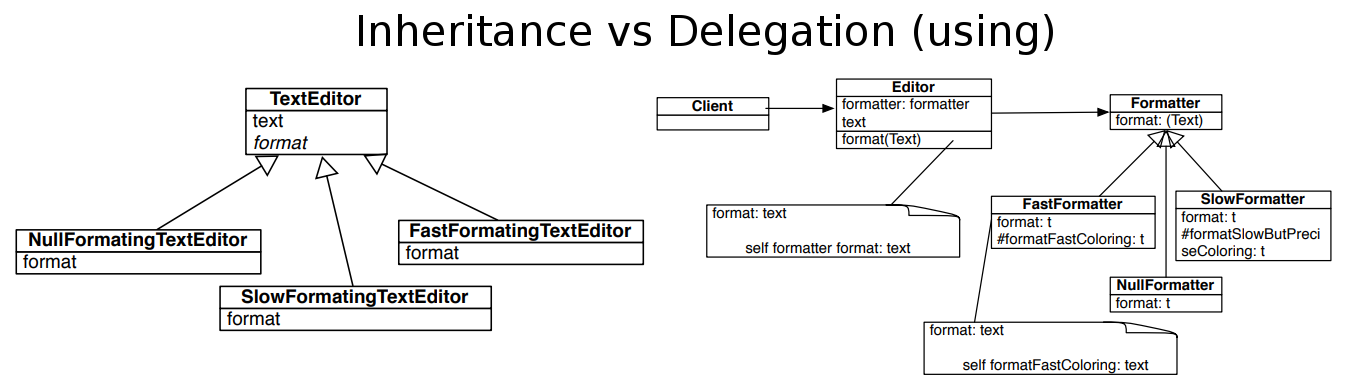
\includegraphics[width=1\textwidth]{topics/bi-wsi-si-10/inheritance-vs-delegation.png}
            \caption{Dědičnost vs. delegování}
      \end{figure}

      \item \textit{Explain the Strategy design pattern.}
      
      \textbf{Strategy pattern} -- definujeme rodinu podobných algoritmů, každý zapouzdříme do své vlastní
      třídy, která poskytuje stejné rozhraní jako ostatní třídy z této rodiny algoritmů.
      Konkrétní algoritmus lze pak měnit za běhu programu.

      \begin{figure}[h]
            \centering
            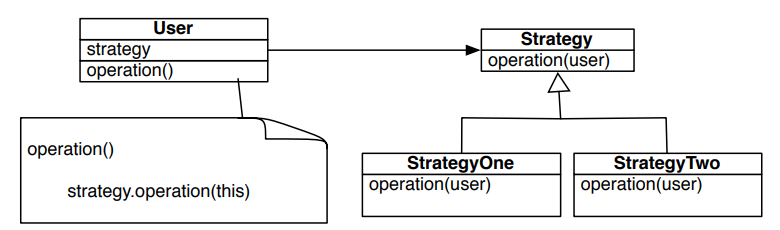
\includegraphics[width=1\textwidth]{topics/bi-wsi-si-10/strategy.png}
            \caption{Strategy pattern}
      \end{figure}

      \item \textit{Explain the Null object pattern, when and how to use it.}
      
      \textbf{Null object pattern} -- jedna z podtříd definuje chování prázdného (\textit{null}) objektu.
      Tímto způsobem lze eliminovat kontrolování \textit{null} hodnoty před každou operací.

      Příklad použití: při implementaci datové struktury binárního stromu lze použít \textbf{null object pattern}
      pro neexistující vrcholy stromu. Vrcholy by pak byly implementovány těmito třídami:

      \begin{itemize}
            \item \textit{TSNode} -- abstraktní třída pro vrchol stromu,
            
            \item \textit{TSBinnaryNode extends TSNode} -- třída reprezentující existující vrchol stromu,
            která obsahuje 3 atributy: \textit{value}, \textit{left}, \textit{right} a na metodu
            \textit{isEmpty()} odpovídá \textit{false},
            
            \item \textit{TSEmptyNode extends TSNode} -- třída reprezentující neexistující vrchol stromu,
            která neobsahuje žádné atributy a na metodu
            \textit{isEmpty()} odpovídá \textit{true}.
            
      \end{itemize}

      \textit{TSEmptyNode} může být \textit{Singleton}, protože instance této třídy nemá žádné vnitřní
      instanční proměnné a proto se všechny instance \textit{TSEmptyNode} chovají stejně. Není tedy důvod
      jich vytvářet zbytečně moc.
      
      \begin{figure}[h]
            \centering
            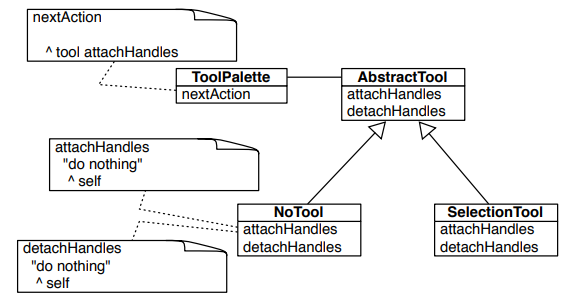
\includegraphics[width=1\textwidth]{topics/bi-wsi-si-10/null.png}
            \caption{Null object pattern}
      \end{figure}

      
      \item \textit{What is dynamic dispatch, explain single and double-dispatch, give examples.}
      
      \textbf{Dynamic dispatch} -- proces výběru implementace polymorfické operace (metody) za běhu programu.

      \textbf{Single dispatch} -- výběr metody je závislý pouze na jednom objektu. Jedná se o klasické
      zaslání zprávy příjemci. Podle toho, kdo je příjemcem se vybere metoda, která se provede.

      \begin{minted}[breaklines]{java}
            receiver.doStuff();
            // podle toho, jakého typu je receiver je vybrána příslušná metoda doStuff()
      \end{minted}

      \textbf{Double dispatch} -- výběr metody je závislý na kombinaci více objektů. Jak funguje
      double dispatch je znázorněno na příkladu se sčítáním hracích kostek. Lze sčítat kostky,
      kostku a pytlíček nebo dva pytlíčky kostek. Výběr prováděné metody závisí jak na typu objektu,
      kterému je zasílána zpráva \textit{sečti}, tak na typu argumentu sčítání.

      \begin{figure}[h]
            \centering
            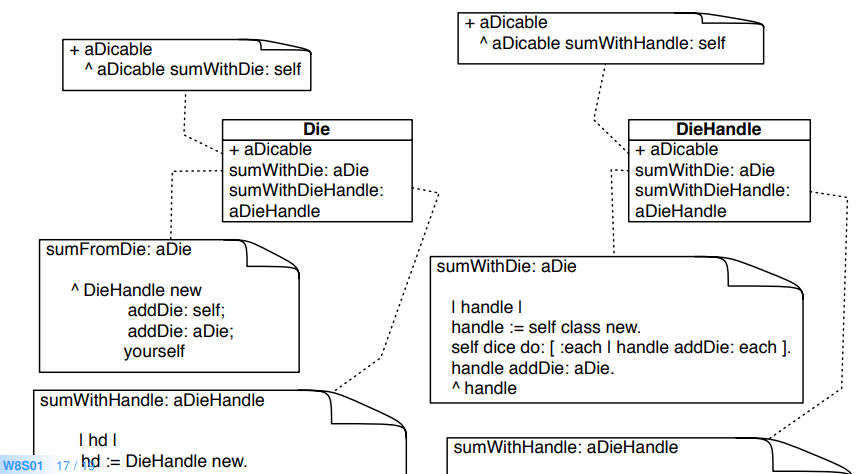
\includegraphics[width=1\textwidth]{topics/bi-wsi-si-10/double-dispatch.png}
            \caption{Double dispatch example}
      \end{figure}

      Celý příklad na \textbf{Double dispatch} lze najít na:

      \textbf{http://rmod-pharo-mooc.lille.inria.fr/OOPMooc/08-MoreOnDispatch/W8S01-Design-DoubleDispatch-Dice.pdf}


\end{itemize}


\end{document}
